\chapter{TINJAUAN PUSTAKA}

% Ubah konten-konten berikut sesuai dengan isi dari tinjauan pustaka
\section{Hasil Penelitian Terdahulu}
Penelitian sebelumnya meneliti bagaimana deteksi objek berbasis \textit{YOLO (You Only Look Once)} terjadi secara \textit{real time} \cite{redmon2016you}. Selain itu, terdapat juga penelitian tentang deteksi postur yoga menggunakan \textit{MediaPipe} \cite{garg2022yoga}. Selanjutnya dibahas deteksi posisi untuk pelatihan dengan \textit{MediaPipe} dan \textit{Machine Learning} \cite{supanich2023machine}. Penggunaan \textit{MediaPipe} juga telah dipelajari untuk memantau latihan bicep curl untuk penguatan otot \cite{nguyen2023assessing}.

  Lalu sebelumnya juga terdapat penelitian terkait mengenai penggunaan model \textit{Faster-RCNN-Inception-V2-COCO} dari \textit{TensorFlow} untuk melakukan pengenalan semaphore bendera . Di Dalam ini Penulis menggunakan \textit{TensorFlow API} dan Model \textit{Deep Neural Network (DNN)} untuk melatih model dan melakukan deteksi gestur semaphore \cite{motty2023flag}


\section{Bendera Semaphore}

\begin{center}
	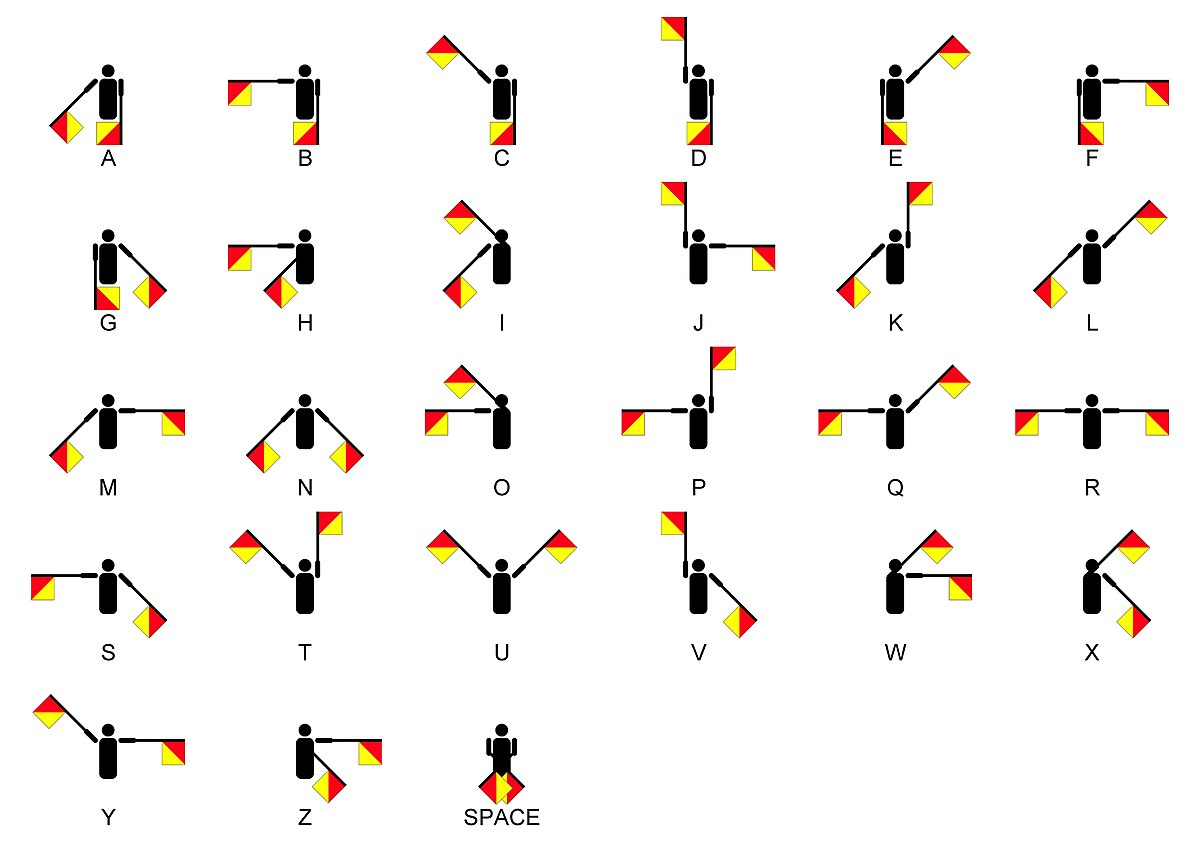
\includegraphics[width=0.9\linewidth]{gambar/bener/Semaphore-Pose.jpg}
	\captionof{figure}{Bendera Semaphore}
	\label{fig:BenderaSemaphore}
\end{center}

Bendera Semaphore adalah sebuah sistem komunikasi yang menggunakan posisi dari dua bendera untuk mengirimkan pesan. Bendera Semaphore pertama kali dikembangkan pada abad ke-18 oleh seorang ahli matematika Prancis bernama Claude Chappe sebagai cara untuk mengirimkan pesan telegraf tanpa menggunakan kabel. \cite{8752707}

Bendera Semaphore menggunakan dua bendera yang dapat digerakkan ke posisi yang berbeda, yang masing-masing mewakili sebuah huruf dari alfabet atau angka. Setiap posisi bendera menunjukkan sebuah karakter yang dapat ditransmisikan kepada penerima pesan. Bendera Semaphore biasanya digunakan untuk mengirimkan pesan jarak jauh, misalnya antar kapal atau antar kota. \cite{gundogdu2019semaphore} 

\section{Estimasi Pose}

Estimasi pose adalah suatu teknik atau metode untuk mengestimasi atau memperkirakan posisi dan orientasi objek dalam ruang tiga dimensi. Pose dalam konteks ini merujuk pada posisi relatif dan orientasi objek terhadap suatu sistem koordinat global. Estimasi pose dapat digunakan dalam berbagai aplikasi, seperti augmented reality, robotika, pemrosesan citra, dan pengenalan gerakan.

Teknik estimasi pose umumnya melibatkan penggunaan data sensor, seperti kamera, sensor inersia, atau lidar. Dalam konteks penggunaan kamera, estimasi pose sering kali mengacu pada perolehan informasi tentang posisi dan orientasi objek berdasarkan analisis citra yang diperoleh dari kamera.

Proses estimasi pose melibatkan beberapa langkah. Pertama, data sensor yang relevan dikumpulkan, seperti gambar dari kamera atau data inersia dari sensor inersia. Selanjutnya, fitur-fitur penting diidentifikasi dalam data sensor, seperti titik-titik referensi, tepi, atau fitur geometris lainnya.

Setelah itu, dilakukan pencocokan atau pembandingan antara fitur-fitur yang terdeteksi dengan fitur-fitur yang diketahui atau telah direkam sebelumnya. Dalam beberapa kasus, estimasi pose juga melibatkan pencocokan dengan model geometris atau model 3D objek yang diketahui. \cite{Andriluka_2014_CVPR}

Estimasi pose melibatkan ekstraksi fitur dari gambar atau video, seperti \textit{keypoints} atau \textit{landmarks}, dan menggunakan fitur-fitur tersebut untuk mengestimasi pose benda atau orang. Ada banyak teknik dan pendekatan yang dapat digunakan untuk estimasi pose, termasuk pendekatan berbasis model, pendekatan berbasis template, dan pendekatan berbasis \textit{Deep Learning}. \cite{Toshev_2014_CVPR}

\section{MediaPipe}
\begin{center}
  % Nama dari file gambar yang diinputkan
  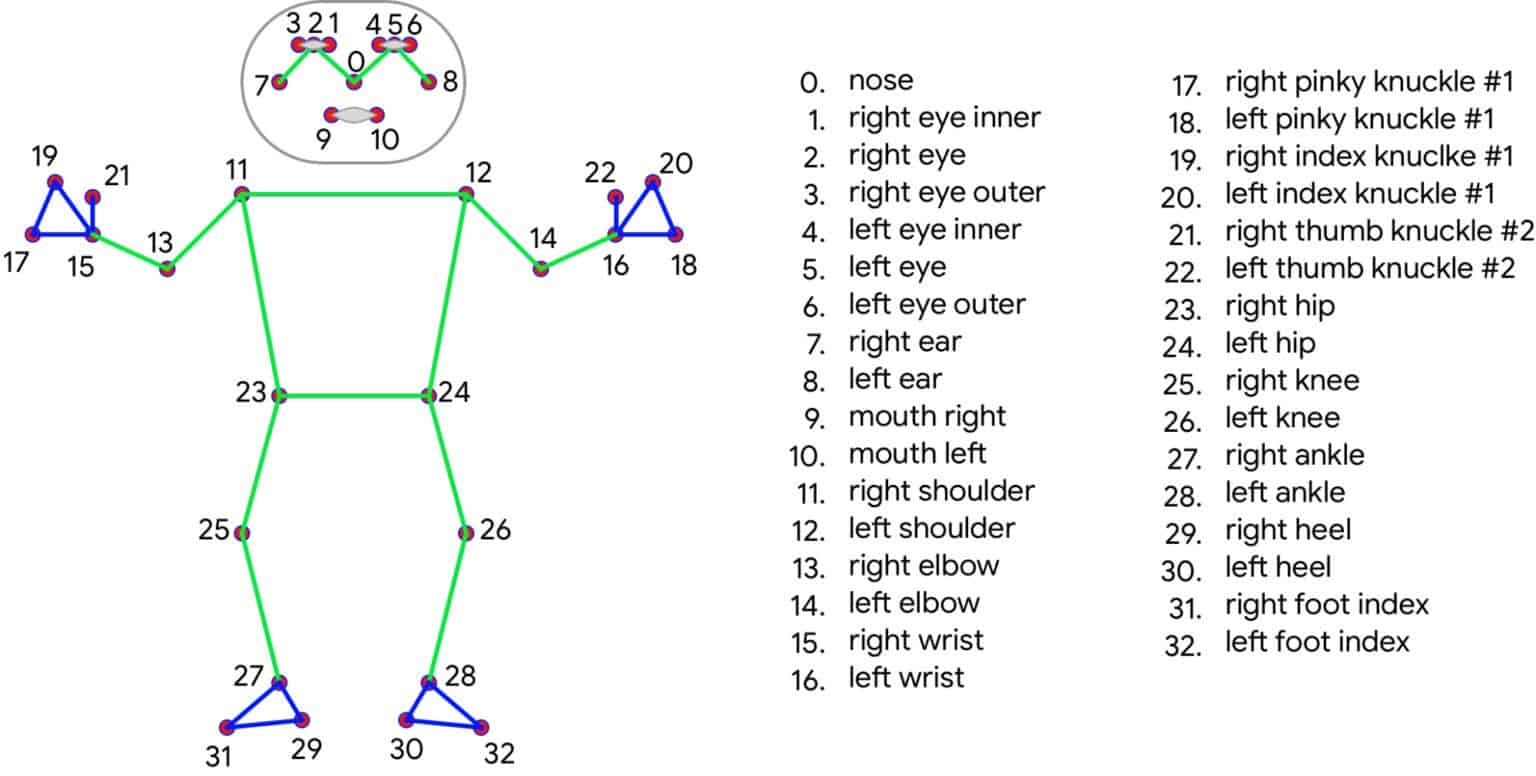
\includegraphics[width=0.8\linewidth]{gambar/humanpose.jpg}
  % Keterangan gambar yang diinputkan
  \captionof{figure}{Arsitektur CNN}
  % Label referensi dari gambar yang diinputkan
  \label{fig:Pose Tubuh dari MediaPipe}
\end{center}

\textit{MediaPipe} merupakan sebuah \textit{framework} yang dikembangkan oleh tim \textit{Google Research} dengan tujuan memproses input sensori seperti video dan audio. \textit{Framework} ini menyediakan kemudahan dan kecepatan dalam menggabungkan komponen-komponen persepsi yang ada maupun baru menjadi prototipe dan mengembangkannya menjadi aplikasi canggih yang dapat dijalankan di berbagai tempat. \cite{lugaresi2019mediapipe}

\textit{MediaPipe} memiliki kemampuan untuk dikonfigurasi sehingga dapat mengelola sumber daya dengan efisien. Hal ini termasuk mengoptimalkan kinerja dengan mengurangi latensi, menangani sinkronisasi data seri waktu seperti frame audio dan video, serta melakukan pengukuran kinerja dan konsumsi sumber daya. Dengan kemampuan ini, \textit{MediaPipe} dapat memberikan performa yang baik dalam memproses input sensori dengan mempertimbangkan keterbatasan sumber daya yang ada.

Salah satu komponen yang dapat dimanfaatkan dalam \textit{MediaPipe} adalah Estimasi Posisi Manusia. Estimasi Pose Manusia merupakan teknik yang bertujuan untuk mendeteksi dan mengidentifikasi posisi tubuh manusia dalam gambar atau video. Dengan menggunakan algoritma dan model yang ada dalam \textit{MediaPipe}, pengembang dapat mengintegrasikan kemampuan ini ke dalam aplikasi mereka.

Dengan adanya Estimasi Pose Manusia, aplikasi yang menggunakan \textit{MediaPipe} dapat melakukan analisis lebih lanjut terhadap posisi tubuh manusia dalam video atau gambar. Hal ini memungkinkan pengembang untuk mengembangkan berbagai aplikasi yang melibatkan interaksi manusia, seperti deteksi gerakan, pengenalan gestur, atau pengukuran postur tubuh untuk keperluan olahraga atau rehabilitasi fisik.

Dengan menggabungkan semua fitur dan kemampuan yang dimiliki oleh \textit{MediaPipe}, pengembang dapat menciptakan aplikasi sensori yang lebih canggih dan memanfaatkan input sensori seperti video dan audio dengan lebih efisien. Framework ini mempercepat proses pengembangan aplikasi lintas platform yang menghadirkan pengalaman interaktif dan berdaya saing tinggi. \cite{singh2021real}

\section{Deep Learning}
\textit{Deep Learning} adalah teknik dalam \textit{Machine Learning} yang memungkinkan model komputasi untuk belajar representasi data dengan berbagai tingkat abstraksi. Metode ini telah meningkatkan secara dramatis kemampuan dalam pengenalan suara, pengenalan objek visual, deteksi objek, dan banyak domain lainnya seperti penemuan obat dan genomika. Deep Learning menemukan struktur yang rumit dalam set data besar dengan menggunakan algoritma \textit{backpropagation} untuk menunjukkan bagaimana mesin harus mengubah parameter internal yang digunakan untuk menghitung representasi di setiap lapisan dari representasi di lapisan sebelumnya. \textit{Deep convolutional nets} telah membawa terobosan dalam pemrosesan gambar, video, suara, dan audio, sedangkan recurrent nets telah menerangi data sekuensial seperti teks dan suara \cite{patterson2017deep}

\begin{center}
	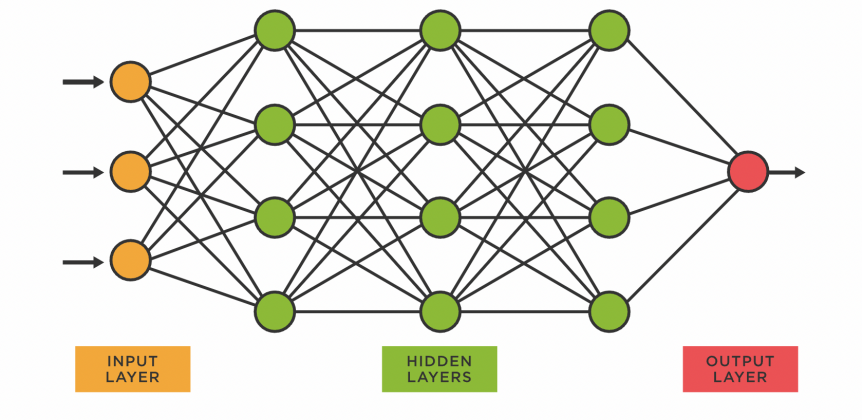
\includegraphics[width=1.0\linewidth]{gambar/bener/ArsitekturDeeplearning.png}
	\captionof{figure}{Deep Learning Layers}
	\label{fig:Deep Learning secara umum}
\end{center}  

\textit{Deep Learning} membuat kemajuan besar dalam memecahkan masalah yang telah menahan upaya terbaik dari komunitas kecerdasan buatan selama bertahun-tahun. Ini ternyata sangat baik dalam menemukan struktur yang rumit dalam data berdimensi tinggi dan oleh karena itu dapat diterapkan ke banyak domain ilmu pengetahuan, bisnis, dan pemerintah. \cite{deng2014deep}

Belajar representasi adalah serangkaian metode yang memungkinkan mesin diberi data mentah dan secara otomatis menemukan representasi yang diperlukan untuk deteksi atau klasifikasi. Metode Deep Learning adalah metode belajar representasi dengan beberapa tingkat representasi, yang diperoleh dengan menyusun modul sederhana tetapi non-linear yang masing-masing mengubah representasi di satu tingkat (dimulai dengan input mentah) menjadi representasi di tingkat yang lebih tinggi, sedikit lebih abstrak. Dengan komposisi cukup banyak transformasi seperti itu, fungsi yang sangat kompleks dapat dipelajari \cite{smith2007teaching}

Salah satu variasi utama dalam Deep Learning adalah \textit{Convolutional Neural Network (CNN)}. \textit{CNN} secara khusus dirancang untuk pengolahan data grid seperti gambar dan video. Struktur konvolusi dalam \textit{CNN} memungkinkan pengenalan pola lokal dalam data dan menghasilkan representasi yang berguna. \textit{CNN} telah menjadi fondasi dalam berbagai tugas penglihatan komputer, termasuk klasifikasi gambar, deteksi objek, dan segmentasi.

Selain \textit{CNN}, ada juga variasi seperti \textit{Recurrent Neural Network (RNN)} yang digunakan untuk memodelkan urutan data, seperti teks dan suara. \textit{RNN} memiliki unit rekurensi yang memungkinkan pengolahan data sekuensial dan mempertimbangkan konteks sebelumnya. Model \textit{RNN} seperti \textit{Long Short-Term Memory (LSTM)} dan \textit{Gated Recurrent Unit (GRU)} telah membantu dalam tugas-tugas seperti pemodelan bahasa alami, pemrosesan bahasa alami, dan pengenalan ucapan.

Selain itu, ada juga arsitektur Deep Learning seperti \textit{Generative Adversarial Networks (GANs)} yang digunakan untuk menghasilkan data baru yang menyerupai data latihan. \textit{GAN} terdiri dari dua jaringan saraf, yaitu generator yang menghasilkan data sintetis dan discriminator yang membedakan antara data sintetis dan data asli. GAN telah digunakan dalam bidang seperti generasi gambar, sintesis suara, dan augmentasi data.

\subsection{Convolutional Neural Network (CNN)}
\begin{center}
  % Nama dari file gambar yang diinputkan
  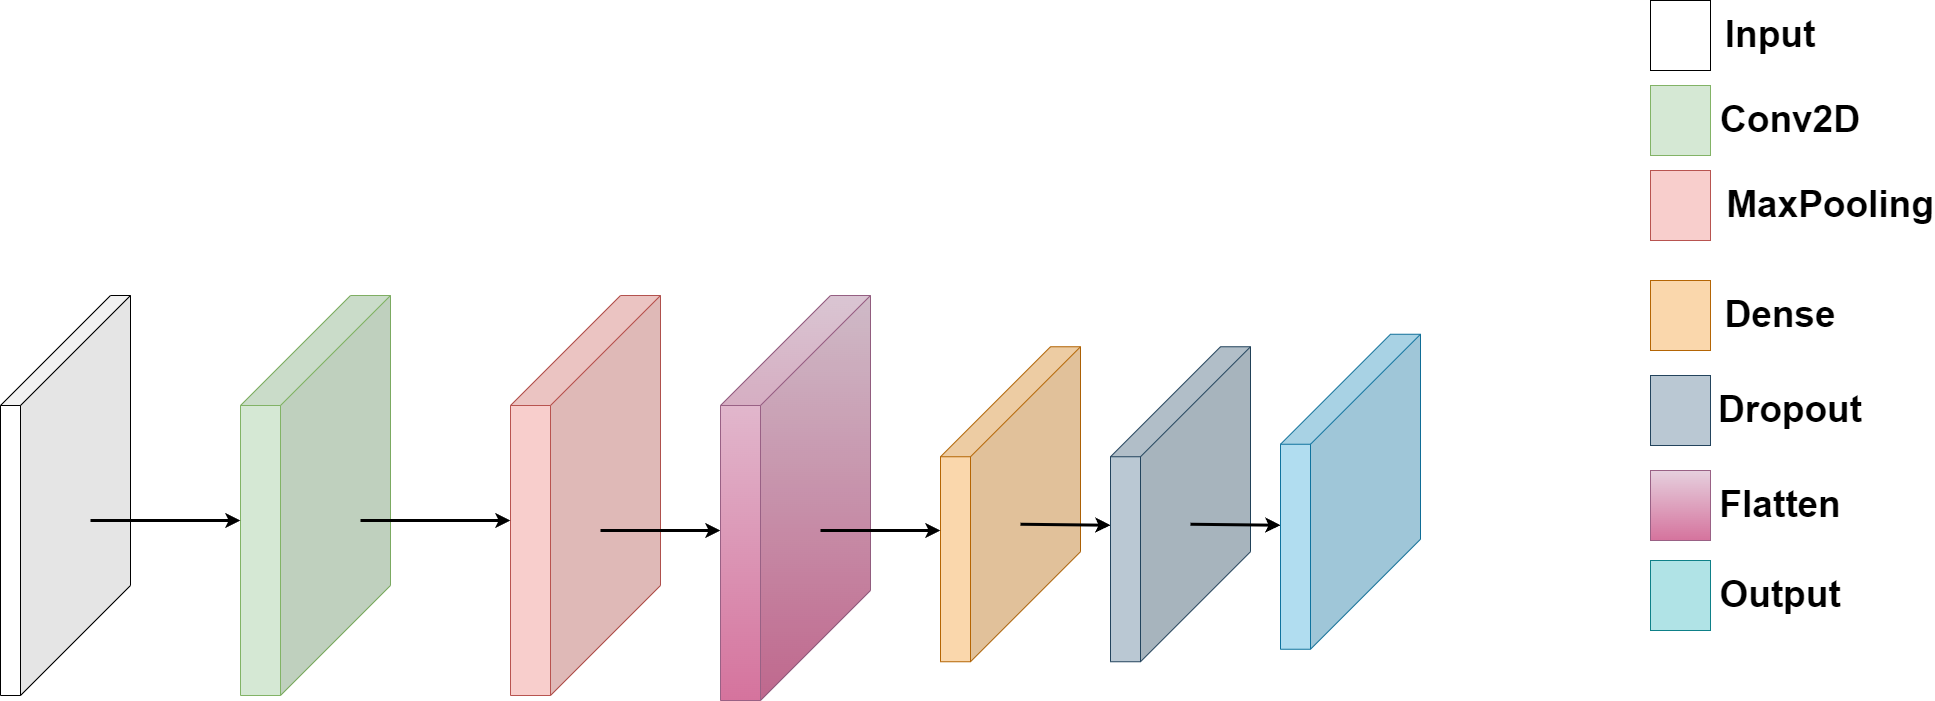
\includegraphics[width=1.0\linewidth]{gambar/bener/Arsitektur_CNN_Umum.png}
  % Keterangan gambar yang diinputkan
  \captionof{figure}{Arsitektur CNN}
  % Label referensi dari gambar yang diinputkan
  \label{fig:Arsitektur Umum Convolutional Neural Network}
\end{center}

\textit{Convolutional Neural Network} merupakan sebuah jenis jaringan saraf tiruan yang sangat efektif dalam mengolah dan menganalisis data dengan struktur spasial, seperti gambar atau video. Arsitektur \textit{CNN} terdiri dari berbagai lapisan yang terdiri dari kumpulan neuron yang saling terhubung melalui bobot dan bias. \cite{wu2017introduction}

Salah satu komponen penting dalam \textit{CNN} adalah operasi konvolusi. Konvolusi melibatkan proses berulang di mana setiap bagian kecil dari input dikenakan pada \textit{filter}, yang merupakan matriks bobot, untuk menghasilkan fitur-fitur lokal yang relevan. Dalam konteks pengolahan gambar, konvolusi memungkinkan \textit{CNN} untuk secara efektif mendeteksi berbagai pola dan fitur visual seperti tepi, sudut, atau tekstur dalam gambar. Operasi konvolusi ini memungkinkan \textit{CNN} untuk memahami struktur spasial data input dengan cara yang sangat efisien.\cite{koushik2016understanding}

Selain konvolusi, \textit{CNN} juga menggunakan operasi maxpooling. \textit{Maxpooling} bertujuan untuk mengurangi dimensi spasial dari setiap fitur yang dihasilkan oleh lapisan konvolusi. Dalam operasi \textit{maxpooling}, blok-blok input yang tumpang tindih diambil nilai maksimumnya, sehingga informasi yang relevan tetap terjaga sementara dimensi data dikurangi. Hal ini membantu dalam mengurangi kompleksitas komputasional dan jumlah parameter yang dibutuhkan oleh jaringan, sambil tetap mempertahankan informasi penting tentang fitur-fitur yang terdeteksi.

Lapisan terakhir dalam arsitektur \textit{CNN} biasanya merupakan lapisan \textit{dense} (sepenuhnya terhubung). Lapisan \textit{dense} terdiri dari neuron-neuron yang saling terhubung sepenuhnya dengan lapisan sebelumnya. Lapisan ini bertujuan untuk menggabungkan dan mengolah fitur-fitur yang telah diekstraksi sebelumnya oleh lapisan-lapisan sebelumnya, sehingga dapat menghasilkan output yang relevan untuk tugas klasifikasi, deteksi objek, atau regresi.

Dengan menggabungkan konvolusi, \textit{maxpooling}, dan \textit{lapisan dense} dalam arsitektur \textit{CNN}, jaringan ini mampu melakukan ekstraksi fitur secara hierarkis, di mana setiap lapisan berkontribusi dalam memperoleh representasi yang semakin abstrak dan informatif dari data input. Inilah yang membuat \textit{CNN} menjadi alat yang sangat efektif dalam berbagai tugas pengolahan gambar dan video, dari pengenalan wajah hingga analisis citra medis.

\subsubsection{ResNet50v2}
\begin{center}
  % Nama dari file gambar yang diinputkan
  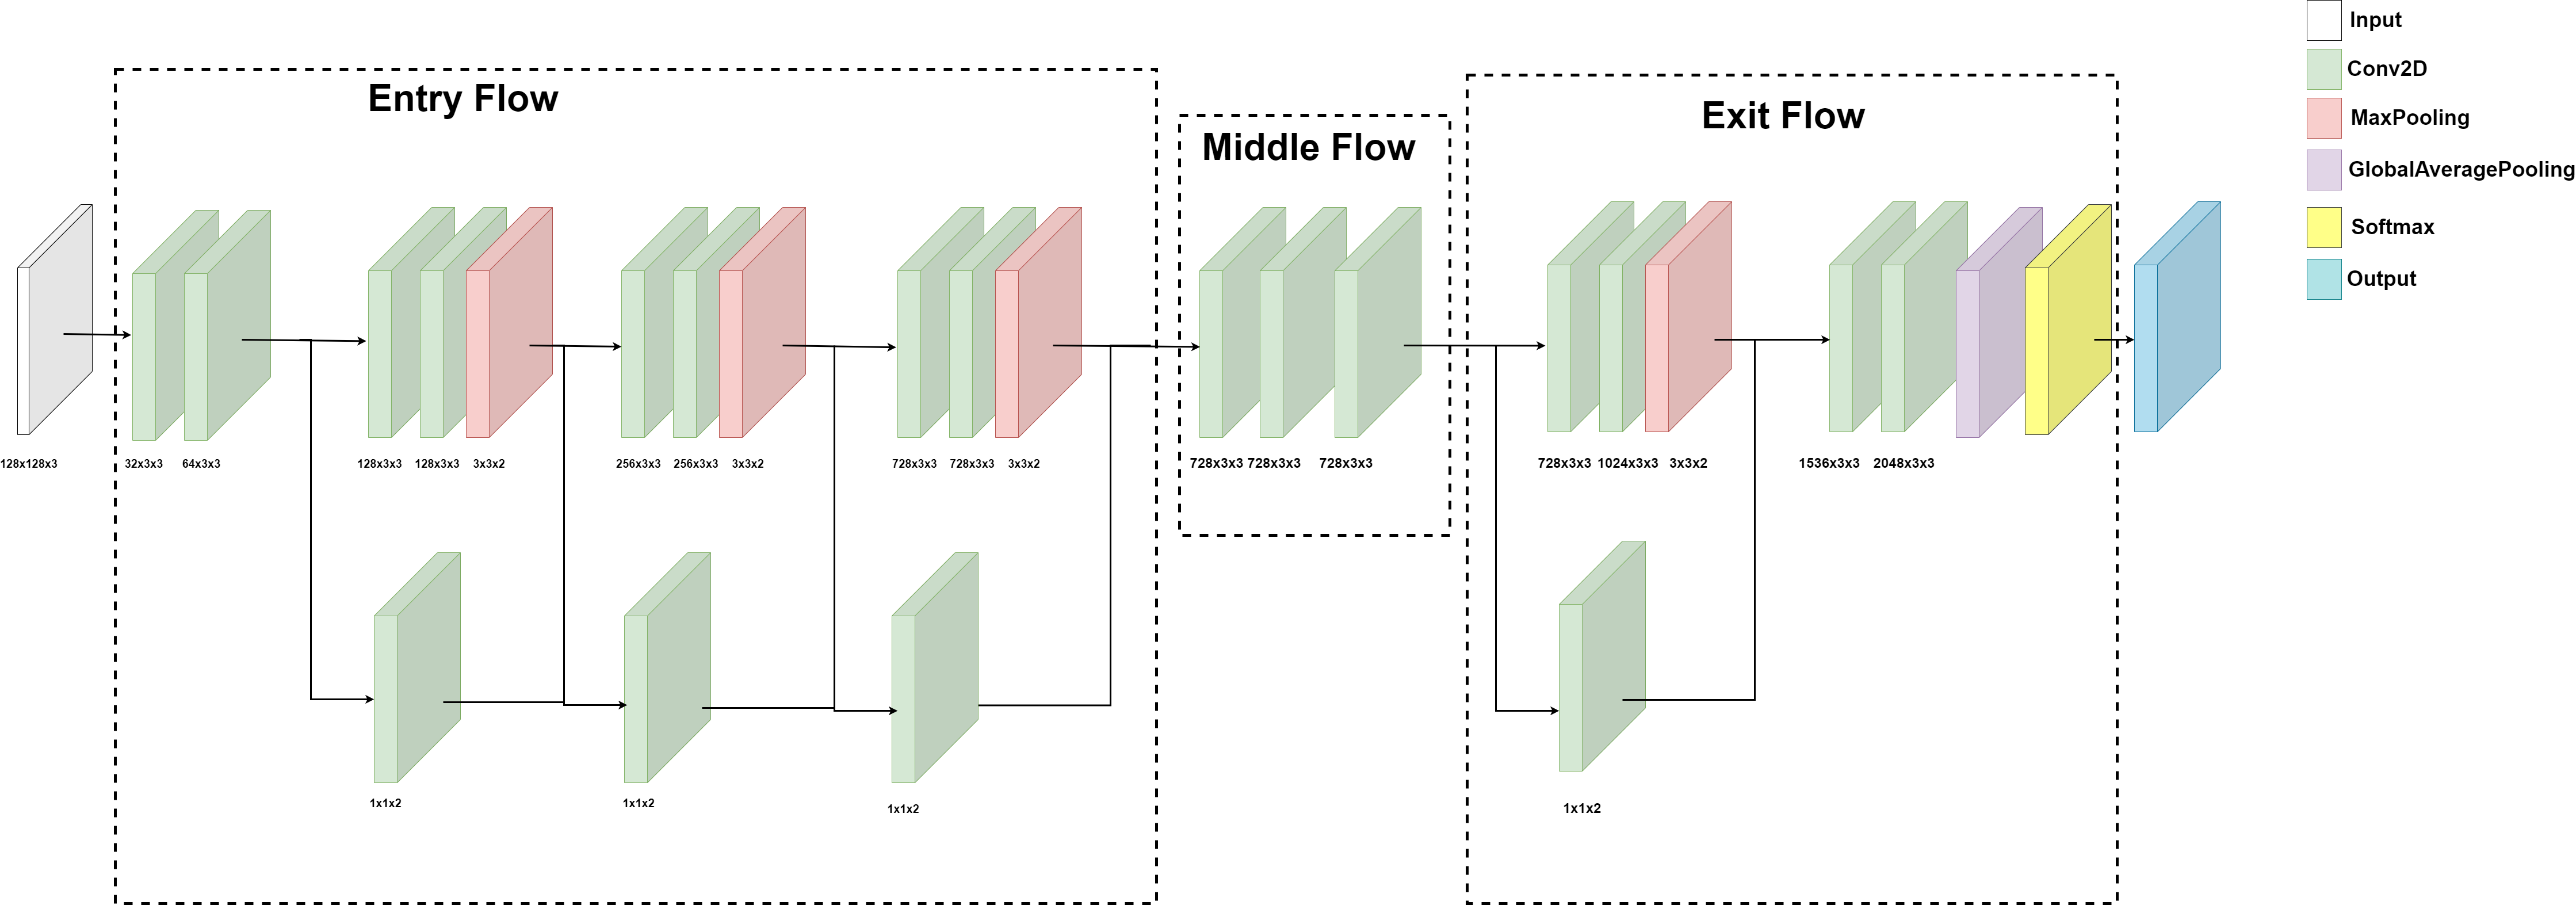
\includegraphics[width=1.1\linewidth]{gambar/bener/Arsitektur_ModelCNNResNet50V2_Dasar.png}
  % Keterangan gambar yang diinputkan
  \captionof{figure}{Arsitektur CNN ResNet50V2}
  % Label referensi dari gambar yang diinputkan
  \label{fig:Arsitektur ResNet50V2}
\end{center}

\textit{ResNet50V2} adalah salah satu model arsitektur jaringan saraf konvolusi \textit{(Convolutional Neural Network/CNN)} yang merupakan versi modifikasi dari \textit{ResNet50}. \textit{ResNet} sendiri merupakan singkatan dari \textit{"Residual Network"} yang dikembangkan oleh Kaiming He dan timnya pada tahun 2015. \textit{ResNet50V2} adalah salah satu varian dari arsitektur ResNet yang memiliki 50 lapisan (layers) dan menggunakan teknik yang disebut \textit{"skip connections"} atau \textit{"residual connections"} untuk mengatasi masalah pemudaran gradien \textit{(vanishing gradient)} yang sering terjadi pada jaringan saraf yang lebih dalam. \cite{rahimzadeh2020modified}

\textit{Skip connections} dalam \textit{ResNet50V2} memungkinkan aliran informasi yang lebih mudah melalui lapisan-lapisan jaringan, dengan cara mengalirkan input langsung ke lapisan-lapisan mendalam atau menambahkan input ke output lapisan tersebut. Hal ini membantu dalam pembelajaran representasi fitur yang lebih baik, mengurangi kemungkinan pemudaran gradien, dan mempercepat pelatihan jaringan.

\textit{ResNet50V2} memiliki beberapa modifikasi dibandingkan dengan \textit{ResNet50} asli. Salah satu modifikasi penting adalah penggunaan \textit{"bottle-neck"} atau blok residual bertingkat. Blok \textit{bottle-neck} ini terdiri dari tiga lapisan konvolusi dengan ukuran kernel yang berbeda, yaitu 1x1, 3x3, dan 1x1, yang mengurangi dimensi fitur dan kompleksitas komputasi pada bagian tengah blok tersebut. Dengan demikian, \textit{ResNet50V2} memiliki struktur yang lebih efisien dan mampu menghasilkan representasi fitur yang lebih kuat dengan pengurangan parameter yang signifikan.

Selain itu, \textit{ResNet50V2} juga menggunakan beberapa teknik lainnya seperti normalisasi batch \textit{(batch normalization)} dan fungsi aktivasi \textit{ReLU (Rectified Linear Unit)} untuk meningkatkan kestabilan dan kemampuan pembelajaran jaringan. \cite{prusty2022resnet50v2}

\subsubsection{Xception}
\textit{Xception} adalah arsitektur jaringan saraf tiruan yang dikembangkan oleh Google Brain dan diperkenalkan oleh François Chollet, pencipta Keras, pada tahun 2017. Xception, yang merupakan singkatan dari \textit{"Extreme Inception"}, adalah variasi dari arsitektur \textit{Inception} yang menggantikan operasi konvolusi standar dalam modul \textit{Inception} dengan konvolusi yang dapat dipisahkan secara mendalam. \textit{Xception} memiliki 36 lapisan dan sekitar 4,3 juta parameter. \textit{Xception} dirancang untuk bekerja dengan gambar berwarna (3 saluran warna) dan mengambil gambar berukuran 299x299 piksel sebagai input.. \cite{chollet2017xception}

\begin{center}
  % Nama dari file gambar yang diinputkan
  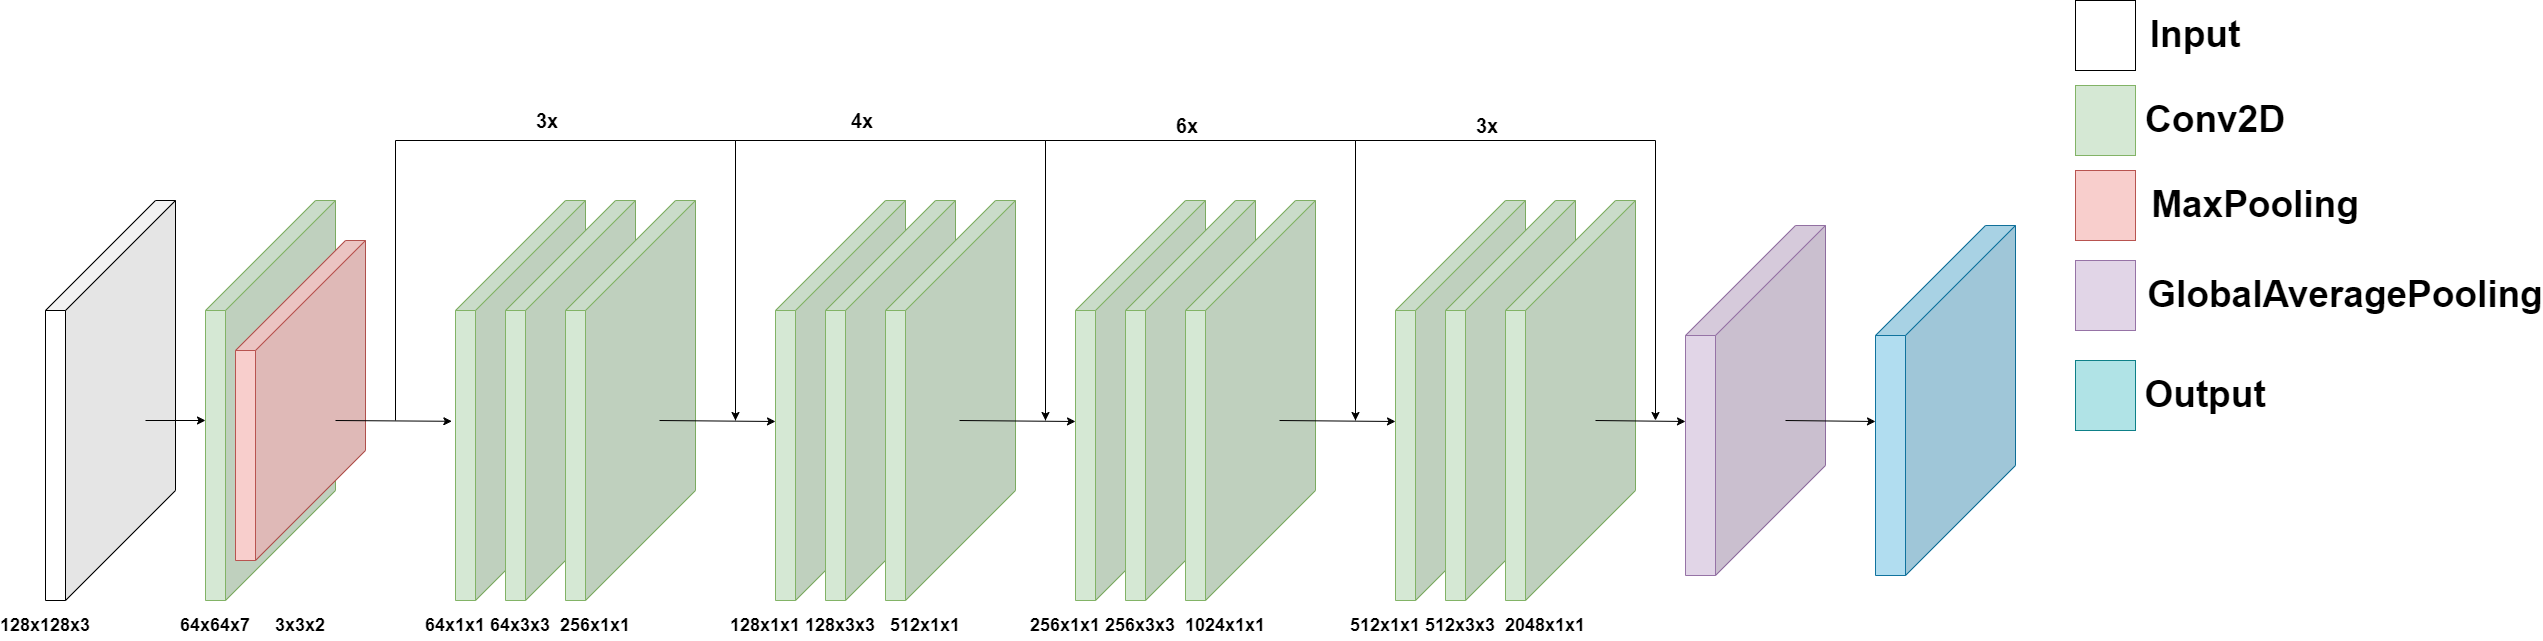
\includegraphics[width=1.0\linewidth]{gambar/bener/Arsitektur_CNNXception.png}
  % Keterangan gambar yang diinputkan
  \captionof{figure}{Arsitektur CNN Xception}
  % Label referensi dari gambar yang diinputkan
  \label{fig:Arsitektur Xception}
\end{center}

Arsitektur ini bergantung pada konsep konvolusi yang dapat dipisahkan secara mendalam. Struktur arsitektur Xception terdiri dari tiga modul utama, yaitu \textit{entry flow, middle flow}, dan \textit{exit flow}. \textit{Entry flow} terdiri dari konvolusi normal diikuti oleh konvolusi yang dapat dipisahkan secara mendalam. \textit{Middle flow} terdiri dari 8 \textit{miniblock}, masing-masing terdiri dari 3 konvolusi yang dapat dipisahkan secara mendalam. Terakhir, \textit{exit flow} terdiri dari konvolusi yang dapat dipisahkan secara mendalam, \textit{feature flattening}, dan \textit{output}.

Konsep konvolusi yang dapat dipisahkan secara mendalam adalah untuk mengurangi jumlah perkalian matriks dalam jaringan, sehingga mengurangi ukuran model. Konvolusi yang dapat dipisahkan secara mendalam melakukan konvolusi dalam dua langkah. Langkah pertama, juga disebut konvolusi depthwise, menggunakan 1 \textit{filter} untuk setiap lapisan input. Output dari langkah ini akan berukuran tinggi x lebar x kedalaman dari gambar asli, asalkan padding digunakan selama konvolusi. Output dari konvolusi depthwise akan menjadi input dari konvolusi \textit{pointwise}. Dalam konvolusi \textit{pointwise}, ukuran \textit{filter} adalah 1x1xkedalaman, di mana kedalaman adalah kedalaman input sebelumnya. Untuk menghasilkan beberapa fitur, lebih dari satu \textit{filter} digunakan dalam proses ini.
\cite{rismiyati2020xception}




